% !TEX options=--shell-escape

\documentclass{article}
\usepackage[utf8]{inputenc}

\usepackage[T2A]{fontenc}
\usepackage[utf8]{inputenc}
\usepackage[russian]{babel}

\usepackage{multienum}
\usepackage{geometry}
\usepackage{hyperref}

\geometry{
 left=1cm,right=1cm,
 top=2cm,bottom=2cm
}
\usepackage{minted}
\usepackage{graphicx}
\graphicspath{ {./images/} }

\title{Алгоритмы и алгоритмические языки}
\author{Лисид Лаконский}
\date{2023 год}

\begin{document}
\raggedright

\maketitle
\tableofcontents
\pagebreak

\section{Алгоритмы и алгоритмические языки — занятие №1}

dll — \textbf{динамически подключаемая библиотека}

Для создания dll в Visual Studio необходимо выбрать шаблон «\textbf{библиотека классов}»

\subsection{Проект «вычисление суммы квадратов двух чисел»}

\subsubsection{Динамическая библиотека}

Для решения поставленной задачи нам необходимо реализовать: \textbf{метод нахождения суммы квадратов двух чисел, метод для ввода данных, метод для вывода данных}

\begin{minted}{csharp}
using System;
using System.Windows.Forms;

namespace ClassLibrary1
{
    public class Class1 {
        public static int Vvod(TextBox t)
        {
            return Convert.ToInt(t.Text);
        }
        public static int Vyvod(TextBox t, int c)
        {
            t.Text = Convert.ToString(c);
        }
        public static int Sum_kv(int x, int y)
        {
            int res = x * x + y * y;
            return res;
        }
    }
}
\end{minted}

В настоящих проектах рекомендуется давать классам, методам, переменным и так далее \textbf{нормальные имена}, а не как в коде выше.

\subsubsection{Основная программа}

Помещаем в форму с помощью вкладки «элементы управления» следующие компоненты: три надписи (\textbf{label}), два поля ввода текста (\textbf{textbox}) и одну кнопку (\textbf{button})

Код собственно программы:

\begin{minted}{csharp}
using System;
// Прочие юзинги...
using LibraryClass1;

namespace ClassProgram1 {
    public partial class Form1 : Form
    {
        public Form1()
        {
            InitializeComponent();
        }
        private void button1_Click(object sender, EventArgs e)
        {
            int a = Class1.Vvod(textBox1);
            int b = Class1.Vvod(textBox2);
            int y = Class1.Sum_kv(a, b);
            Class1.Vyvod(textBox3, y);
        }
    }
}
\end{minted}

\pagebreak
\section{Алгоритмы и алгоритмические языки — занятие №2}

\subsection{Разветвляющийся алгоритм}

Алгоритм называется разветвляющимся, если последовательность выполнения его шагов изменяется в зависимости от некоторых условий (логических выражений, которые могут принимать одно из двух значений – \textbf{истина} и \textbf{ложь}).

Пример с паролем — \textbf{простой условный оператор}:

\begin{center}
    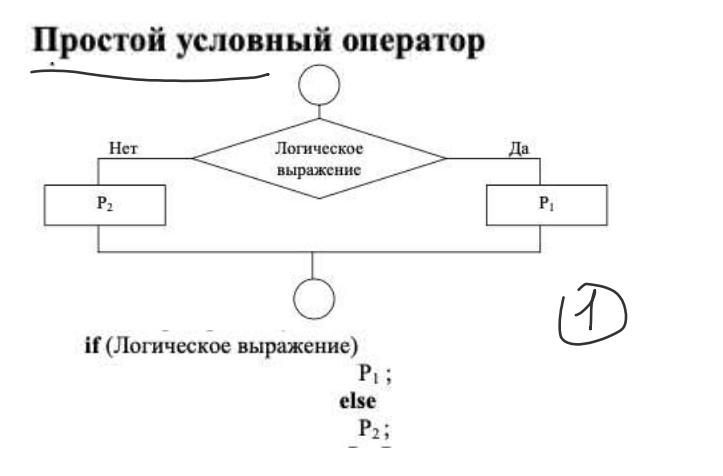
\includegraphics{images/image_00.png}
\end{center}

\pagebreak
Пример с возрастом — \textbf{многозначные ветвления}:

\begin{center}
    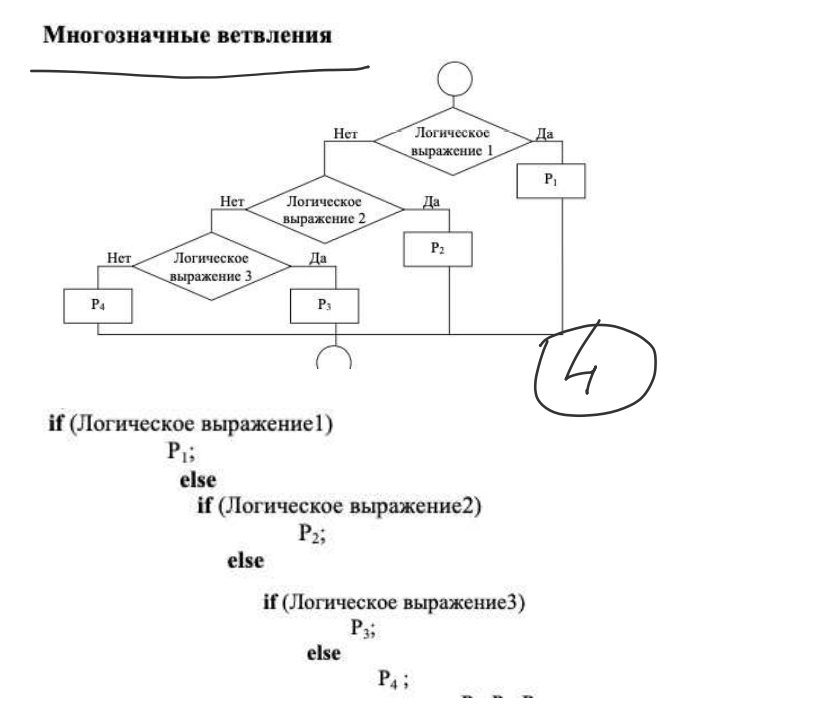
\includegraphics[width=\textwidth]{images/image_01.png}
    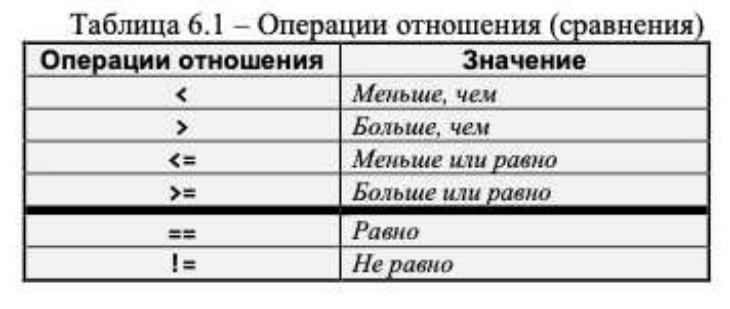
\includegraphics[width=\textwidth]{images/image_02.png}
    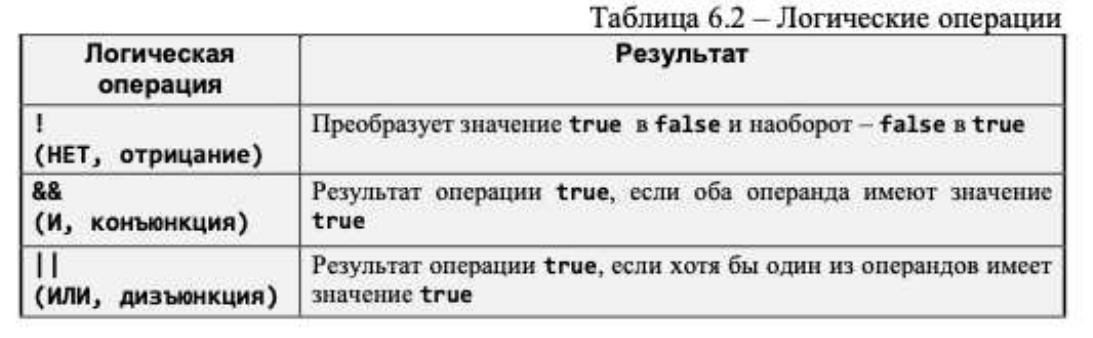
\includegraphics[width=\textwidth]{images/image_03.png}
    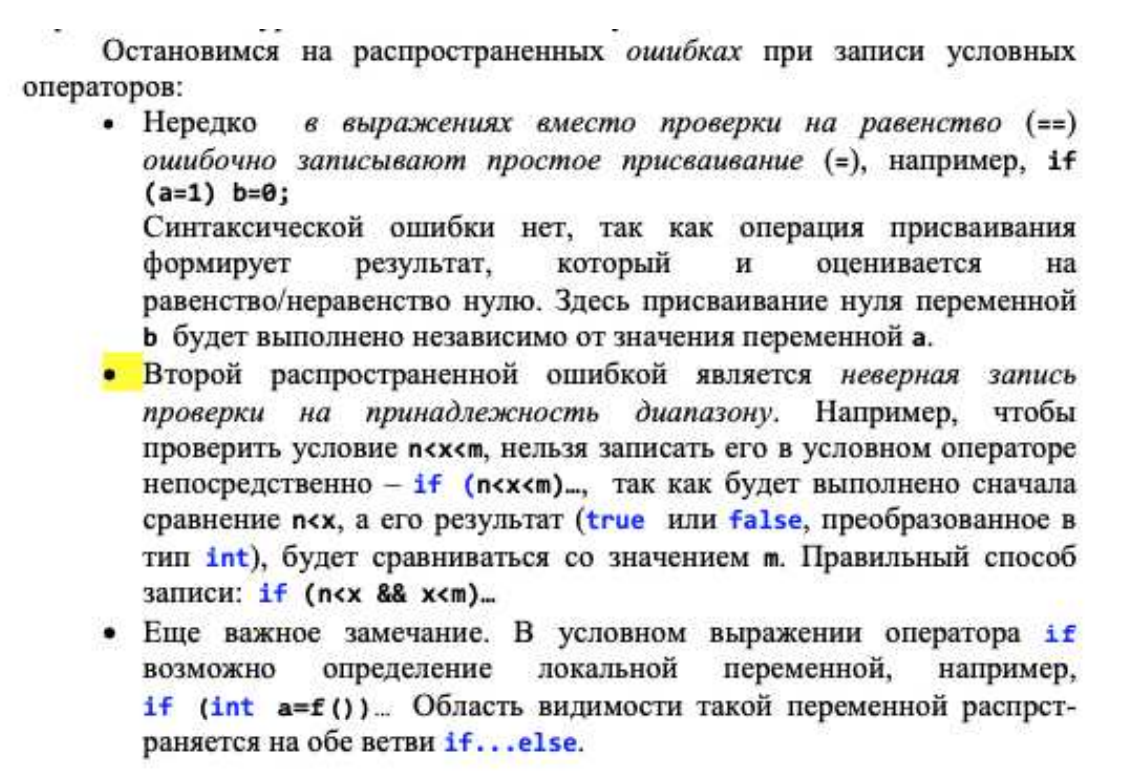
\includegraphics[width=\textwidth]{images/image_04.png}
\end{center}

\pagebreak
\section{Алгоритмы и алгоритмические языки — занятие №3}

В лабораторной работе следует использовать три TextBox для организации ввода данных, кнопку, табличный компонент для вывода таблицы. В таблице должно быть два столбца: «икс» и «игрек».

Виды:

\begin{multienumerate}
    \mitemxxx{Сумма}{Количество}{Максимальное и минимальное}
    \mitemxx{Произведение}{Ничего кроме таблицы}
\end{multienumerate}

Пять методов. В dll-библиотеке должны быть методы за все лабораторные работы — ввод, вывод, метод расчета выражений.

Метод для вывода результатов табулирования функции в табличный компонент:

\begin{minted}{csharp}
public static void _ (double x, double y, DataGridView DGV) {
    DGV.Rows.Add(x.ToString(), y.ToString());
}
\end{minted}

Схемы должны быть выполнены согласно требованиям ГОСТ.

Циклы — с известным и неизвестным количеством повторений.

\pagebreak
\section{Алгоритмы и алгоритмические языки — занятие №4}

Через какое-то время будет ещё одна контрольная работа по 3 и 4 лабораторной работе.

«Создание приложения с итеративной циклической структурой»

Виды циклов:

\begin{multienumerate}
    \mitemxxx{for}{while}{do.. while}
\end{multienumerate}

Выведение рекуррентной формулы.

При суммировании ряда необходимо решать следующие задачи:

\begin{enumerate}
    \item Свести вычисления к простейшим арифметическим операциям
    \item Уменьшить число этих операций и время расчёта
    \item Уменьшить погрешность округлений
\end{enumerate}

Источники погрешностей:

\begin{enumerate}
    \item Ошибки в исходных данных
\end{enumerate}

Задачи сокращения количества операций и уменьшения погрешности вычислений решает рекуррентная формула, позволяющая вычислить значение очередного члена ряда, используя уже найденные значения предыдущего.

Рекуррентная формула имеет вид:

$$
a_{n + 1} = a_{n} * \ln n!
$$

\pagebreak
\section{Алгоритмы и алгоритмические языки — занятие №5}

Синтаксис определения одномерного массива: тип данных[] имя массива = new тип данных[общее количество элементов массива]

Второй вариант: тип данных[] имя массива

\hfill

Для вывода должны использоваться элементы DataGridView и MessageBox, TextBox использовать запрещено.

\hfill

ColumnHeadersVisible — параметр для заголовков столбцов.

В таблице индексы должны располагаться в нулевой строке.

AutoScaleColumnsMode -> AllColls, AutoSizeRowsMode, DefaultCellStyle.

Всё это для исправления негибкости таблицы под размеры DataGridView.

\hfill

\begin{center}
    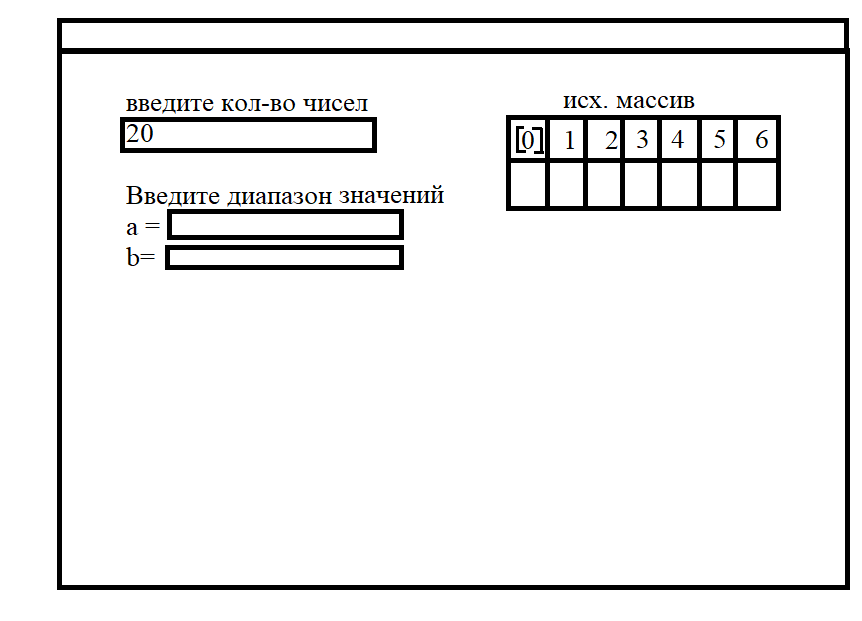
\includegraphics[width=\textwidth]{images/image_05.png}
\end{center}

Дополнительной подпрограммы для результирующего массива не нужно — также использовать output\_mas.

Для решения задачи чаще всего достаточно одного метода.

\begin{enumerate}
    \item Enter\_mas — генерирует элементы массива
    \item Output\_mas – вывод элементов массива на элемент DataGridView
    \item Метод ввода – для конвертации строкового значения в числовое
\end{enumerate}

На примере задачи нахождения чисто положительных чисел:
Методы выше

\begin{minted}{csharp}
public static int kol(int[] mas, int length) {
    int count = 0;
    for (int i = 0; i != length; ++i) {
        if (mas[i] > k)
            count++;
    }
    return count;
}
\end{minted}

Вопрос для зачёта: какие в C\# какие бывают методы? Вопрос(ы) могут повторяться. Если метод считает одно значение – использовать return.

\pagebreak
\section{Алгоритмы и алгоритмические языки — занятие №6}

Проблемы с set\_mas не такие страшные – изменять можно, пусть и желательно соблюдать структуру.

\hfill

Шестая работа – продолжение пятой работы.
В задание шестой работы вставить задание из лабораторной работы №5. Перечисляем алгоритмы, которые нам необходимо реализовать.

Перечисляем методы (по подсчётам Сергея Ростиславовича – 3-4). Вывод в MessageBox. Рисовать прямоугольником такой вывод – неправильно, он рисуется параллелограммом (вывод по ГОСТу), где писать не всю строчку кода, а просто «Вывод // Что выводится, необязательно со словом вывод, можно просто «Нет таких чисел».

\hfill

Ничего переставлять и убирать в алгоритмах не надо. Блок-схемы там не всегда верны, периодически сделаны по устаревшим ГОСТам.

Циклы тут часто начинаются с единицы. Учесть, что индексация массивов начинается с нуля, так что, очевидно, слегка изменить код под это.

К каждому методу давать комментарии с кратким пояснением, что это такое.

\hfill

Если в пятой лабораторной работе массив выходит результирующим – то сортировать алгоритмами именно его. В противном случае – изначальный. Сортировка и изначальная задача, желательно, по одной кнопке. Методы излагать в логической последовательности.

Основная ошибка – вылет индекса за пределы размера массива.

\hfill

\begin{minted}{csharp}
public static void Insert(int [] mas, int length, int poz, int chislo) {
    for (int i = length – 1; i >= poz; i--) { // цикл по убыванию
        mas[i + 1] = mas[i];
        mas[i] = chislo;
    }
}
\end{minted}

Событийная кнопка:

\begin{minted}{csharp}
Button1_Click() {
    Int length = ...
    Int[] arr = new int[length];
    Int A = ...
    Int B = ...
    Enter_mas();
    Output_mas();
    String chislo_ = Microsoft.VisualBasic.Interaction.InputBox(
        "Введите число для добавления в массив", "Ввод", "", ...
    );
    String poz = Microsoft.VisualBasic.Interaction.InputBox...
    Class1.Insert(arr, length,  poz, chislo_);
    Class1.Output_mas(arr, length + 1, dataGridView2);
}
\end{minted}

Если VisualBasic не работает, то нужно добавить ссылку на него в проект.

\begin{minted}{csharp}
public static void Resize(ref int[] mas, int new_size) {
    Int[] newArr = new int[newSize];
    for (int i = 0; i < arr.length; i++) 
        newArr[i] = mas[i];
    mas = newArr;
}
\end{minted}

\pagebreak
\section{Алгоритмы и алгоритмические языки — занятие №7}

\subsection{Работа с двумерными массивами}

Надо относиться к творчески. Некоторым образом можно менять задания, если они как-то слишком неудобны.

Ещё 1 лекция. 7 июня лекции не будет. 6 июня – защита курсовой работой. Чуть раньше – зачёт.

\hfill

\textbf{Обязательно} скопировать индивидуальные задачи в пункт 4.1, правильными словами описать свой функционал.

Не писать разработку конспекта и системы тестирования как функционал. Лишь доп. задачи и собственную дополнительную функциональность. Оптимизировать пункт 2.3 под это.

В случае ухода на перезачёт – в ЭОС будет прикрепление со сдачей доработок за лето.

\hfill

Следует создать новую, последнюю на семестр DLL-библиотеку. Второе прикрепление лабораторных работ к 20 мая. Последний этап будет накануне зачёта. Возможно, стоит всё перепечатать. Реализация алгоритмов с двумерными массивами – необязательна к этому этапу, потому что мало времени. Базовые алгоритмы обработки массивов вообще не выложены.

\begin{enumerate}
    \item $i = j$ — главная диагональ
    \item $i > j$ — ниже главной диагонали, $i < j$ — выше главной диагонали
    \item $i + j - 1 = n$ — побочная диагональ
    \item $i + j - 1 < n$ — выше побочной диагонали, $i + j - 1 > n$ — ниже побочной диагонали
\end{enumerate}

Синтаксис вложенного цикла:

\begin{minted}{csharp}
for (i = n1; i <= n2; ++i) {
    for(j = m1; j <= m2; ++j) {
        P1;
        P2;
        ...
        Pn;
    }
}
\end{minted}

Пример вложенного цикла:

\begin{minted}{csharp}
int a = 5;
for (int i = 1; i != 2; ++i) {
    for (int j = 1; j <= 2; ++j) {
        a = a + 5;
    }
}
\end{minted}

На зачете может понадобиться построить таблицу с раскрытием изменения параметров в цикле.

\hfill

Общий вид объявления двумерного массива: тип данных [,] имя массива = new тип данных[кол-во строк, кол-во столбцов];

Пример:

\begin{minted}{csharp}
int[,] a = new int[4, 4];
\end{minted}

\hfill

DataGridView при выводе в интерфейс подтянуть под 5х5 матрицу. Убрать пустые строки и пустые столбцы.

Перед решением задачи, очевидно, убедиться, что массив на экране, и потом решать.

К зачёту скачать visual studio 2010 и потренироваться в нём, потому что если на зачёте дадут что-то писать – будет именно visual studio 2010.

Все работы иметь с собой. Сообщения выводить в MessageBox. Ввод в текстовые поля легче всего делать с помощью InputBox.

\pagebreak

Код событийной кнопки:

\begin{minted}{csharp}
Private void button1.Click() {
    int A = Class1.Vvod(textBox1);
    int B = Class1.Vvod(textBox2);
    int [,] arr = new int[A, B];
    Class1.ArrayGenerate(arr, A, B);
    Class1.Output_mas(arr, A, B, dataGridView1);
    int K = Class1.Kol(arr, A, B);
    int[] rezarr = new int[K];  
    MessageBox.Show("Кол-во полезных элементов" + K, ...);
    Class1.Set_rezmas(arr, rezarr, A, B, K, out int g_;
    Class1.Output_mas(rezarr, g, dataGridView2);
}
\end{minted}

Перепись задания – полностью.

Пропуски и недописки в записи во внешние программы – частично дополнять из кода к одномерным массивам, + свои названия и прочее. 

\pagebreak
\section{Алгоритмы и алгоритмические языки — занятие №8}

Вместо лекции 07.06 – зачёт у первой группы. Можно подводить итоги.

Основные требования к выпускной квалификационной работе – пятый раздел.

Иметь с собой промежуточные зачеты. Вопросы к зачету: первые 20 легкие, оставшиеся 29 — для злостных прогульщиков. Зачет безоценочный, поэтому не страшно ответить не на все.

С собой иметь dll-шаблон для вывода одномерного и двумерного массива в DataGridView. Очень важно, время строго ограничено, поэтому методы вывода массивов на экран очень сильно упростят жизнь.

Некоторым будут даваться дополнительные задачия. На всякий случай принести электронные проекты курсовых работ на флешке.

\hfill

Создание setup-файла. Необязательно к курсовой работе, но желательно. В меню Visual Studio пункт «Расширения»—«Управление расширениями»

Нажать в обозревателе решений по проекту и нажать «Добавить проект». В строке «Поиск шаблонов», там найти через ключевые слова setup.

\begin{center}
    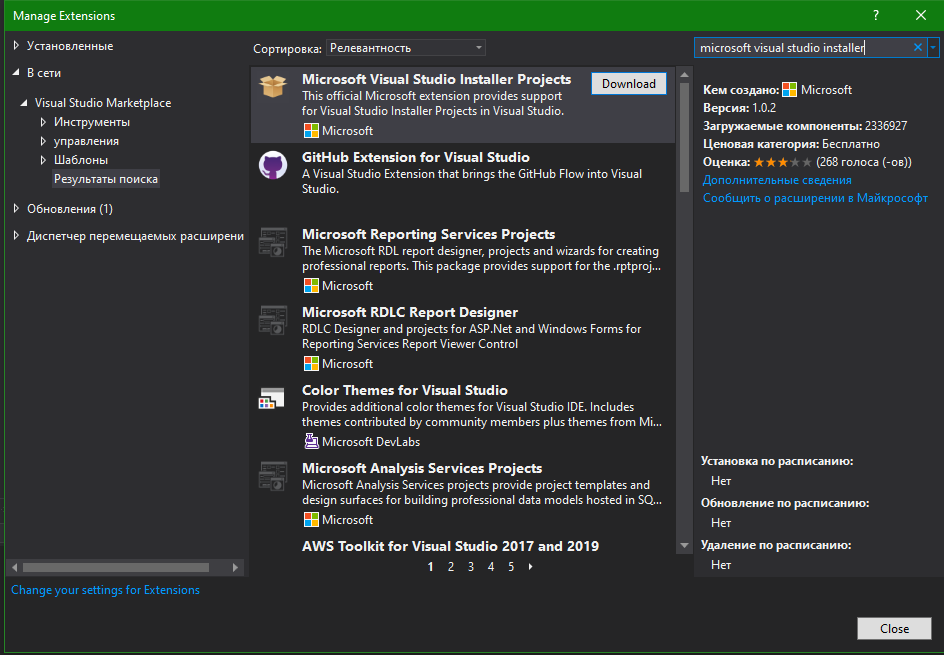
\includegraphics[width=\textwidth]{images/image_06.png}
\end{center}

\begin{enumerate}
    \item Application Folder – папка установки программы
    \item User’s Desktop – буквально рабочий стол пользователя
    \item User’s Program Menu – меню в папке пуск
\end{enumerate}

Добавление выходной группы проекта – просто нажать OK. Просьба о создании ярлыка. Потом как-то перетащить его в user desktop. Правой кнопкой мыши и командой app добавляем папку внутрь Program menu, даём ей имя.

Суть записи функционала в 2.3 – описать в том числе и как оно делается. То есть создавая setup-файл – не просто показать работу setup файла, но и заснять процесс его создания.
    
\end{document}